\documentclass{article}
\usepackage{xparse}
\usepackage{tikz}

\usetikzlibrary{shapes.multipart,calc}
\newcommand{\npd}{\nodepart{two}}
\newcommand{\npt}{\nodepart{three}}
\newcommand{\npq}{\nodepart{four}}
\newcommand{\npc}{\nodepart{five}}

\tikzset{fnode/.style={rectangle split, rectangle split part align={left,left,left,center,left}, rectangle split parts=5, draw, minimum width =2.75cm, rounded corners}}

\tikzset{label style/.style={draw, rounded corners}}

\NewDocumentCommand{\anchormark}{O{0.15 cm} m O{0.05}}{%
        \tikz[overlay,remember picture,baseline=-0.5ex,xshift=#1] \node[draw,fill=black,circle,scale=#3] (#2) {};
}

\begin{document}
\thispagestyle{empty}
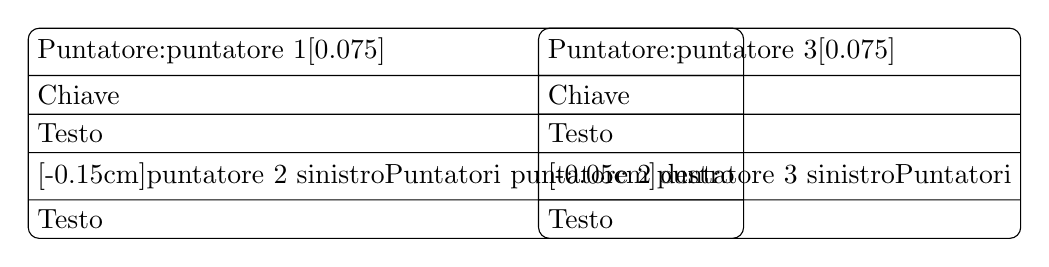
\begin{tikzpicture}[remember picture]
\node[fnode] (r1) at (0,0) {Puntatore:\anchormark{puntatore 1}[0.075]  \npd Chiave  \npt Testo \npq \anchormark[-0.15cm]{puntatore 2 sinistro}Puntatori \anchormark{puntatore 2 destro}\npc Testo};  
\node[fnode] (r2) at (5,0) {Puntatore:\anchormark{puntatore 3}[0.075]  \npd Chiave  \npt Testo \npq \anchormark[-0.05cm]{puntatore 3 sinistro}Puntatori\npc Testo};  
\end{tikzpicture}
\begin{tikzpicture}[remember picture,overlay,-stealth] 
\draw (puntatore 1.center) to ($(puntatore 1.center)+(2,1)$) node[right,label style] (mylabel){label};
\draw (puntatore 2 destro.center) to (puntatore 3 sinistro);
\draw (puntatore 2 sinistro.center) to ($(puntatore 2 sinistro.center)+(-1,1)$)node[left,label style]{label};
\draw (puntatore 3.center) |-(mylabel);
% just to connect r1 and r2
\draw(r1.south)|- ($(r1.south)!0.5!(r2.south)-(0,1)$)-|(r2.south);
\end{tikzpicture}
\end{document}
